\documentclass{standalone}
% translate with >> pdflatex -shell-escape <file>

% This file is an extract of the PGFPLOTS manual, copyright by Christian Feuersaenger.
% 
% Feel free to use it as long as you cite the pgfplots manual properly.
%
% See
%   http://pgfplots.sourceforge.net/pgfplots.pdf
% for the complete manual.
%
% Any required input files (for <plot table> or <plot file> or the table package) can be downloaded
% at
% http://www.ctan.org/tex-archive/graphics/pgf/contrib/pgfplots/doc/latex/
% and
% http://www.ctan.org/tex-archive/graphics/pgf/contrib/pgfplots/doc/latex/plotdata/

\usepackage{pgfplots}
\pgfplotsset{compat=newest}

\pagestyle{empty}

\begin{document}
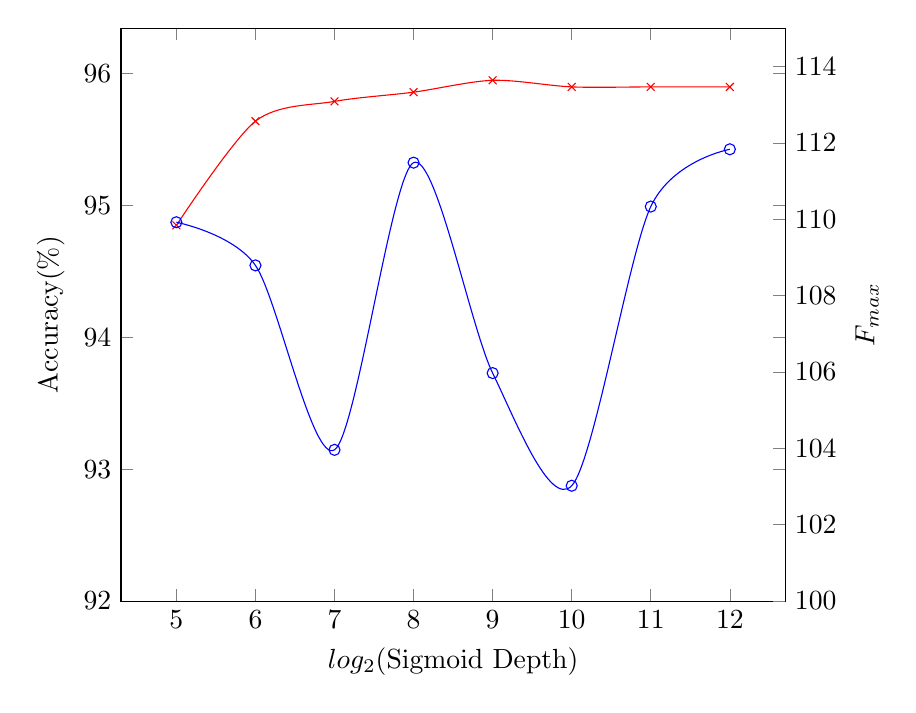
\begin{tikzpicture}
\begin{axis}[
    scale only axis,
    xlabel=$log_2$(Sigmoid Depth),
    ylabel=Accuracy(\%),
    legend style={at={(0.7,0.15)},
    anchor=north,legend columns=-1},
    xtick={0,5,6,7,8,9,10,11,12},
    ymin = 92]
\addplot[smooth,color=red,mark=x] coordinates {
	(5,   94.85)
	(6,   95.64)
	(7,   95.79)
	(8,   95.86)
	(9,   95.95)
	(10,  95.90)
	(11,  95.90)
	(12,  95.90)
};

\end{axis}


\begin{axis}[
    scale only axis,
    ymin=100,ymax=115,
    axis y line*=right,
    axis x line=none,
    ylabel=$F_{max}$]
    \addplot[smooth,color=blue,mark=o] coordinates {
	(5,   109.92)
	(6,   108.79)
	(7,   103.96)
	(8,   111.48)
	(9,   105.97)
	(10,  103.02)
	(11,  110.33)
	(12,  111.83)
   };

  \end{axis}


\end{tikzpicture}
\end{document}
